\section{Framework Grundlagen}

\begin{itemize}
	\item OO Klassen die Zusammenarbeiten
	\item Verfügt über Erweiterungspunkte / Hooks
	\item Steuert den Kontrollfluss (im Gegensatz zu einer Library); ``main()'' lebt im Framework \\
		``Hollywood Principle: Don't call us, we call you''
	\item Stellt nützliche Klassen zur Verfügung
\end{itemize}

\textbf{Vorteile}

\begin{itemize}
	\item Weniger Aufwand für Applikationsentwicklung, da viel wiederverwendet werden kann
	\item Zuverlässiger und robuster Code, falls Framework breit eingesetzt
	\item Applikationscode wird konsistenter und modular strukturiert
	\item Probleme der Kompatibilität sind oft schon gelöst
	\item Verbesserte Integration von ähnlichen Applikationen (Produktfamilien wie MS Office)
\end{itemize}

\textbf{Nachteile}

\begin{itemize}
	\item Anbindung ans Framework meist über Vererbung; stärkste Form von Koppelung
	\item Lock In Gefahr wegen hoher Koppelung (ein dünner Entkopplungslayer kann eigene Komponenten vom Framework trennen)
	\item Komponente von Frameworks können oft nicht ohne das Framework verwendet werden
	\item ``Frameworkers Dilemma'': Ein Framework wächst nicht / wird nicht weiterentwickelt weil es niemand benutzt oder weil es benutzt wird und Änderungen Probleme bei den bestehenden Applikationen verursachen kann
\end{itemize}

\textbf{Entwurf eines Frameworks}

\begin{itemize}
	\item Einfache Interfaces sind in der Regel stabiler
	\item Flexible Interfaces ebenfalls
	\item Nutze Konfiguration um direkte Code Abhängigkeiten zu verringern
	\item Benutze geeignete Patterns, z.B. Extension Interface
\end{itemize}

\textbf{Application Frameworks}

Dienen zur Wiederverwendung von Infrastruktur für ähnliche Applikationen in einem gemeinsamen Kontext.

Die Entwicklung ist oft Evolutionär und wird von einigen konkreten Applikationen getrieben, von denen Gemeinsamkeiten ins Framework übertragen werden.

\textbf{Micro Frameworks}

Einige Pattern stellen Micro Frameworks mit Erweiterungspunkten, Hooks und der Steuerung des Kontrollflusses dar.

\begin{itemize}
	\item Template Methods - Die Template Method in der AbstractClass steuert den Kontrollfluss; Die PrimitiveOperations bilden Hook Methods
	\item Strategy - ...
	\item Command Processor

	\begin{figure}[H]
		\centering
		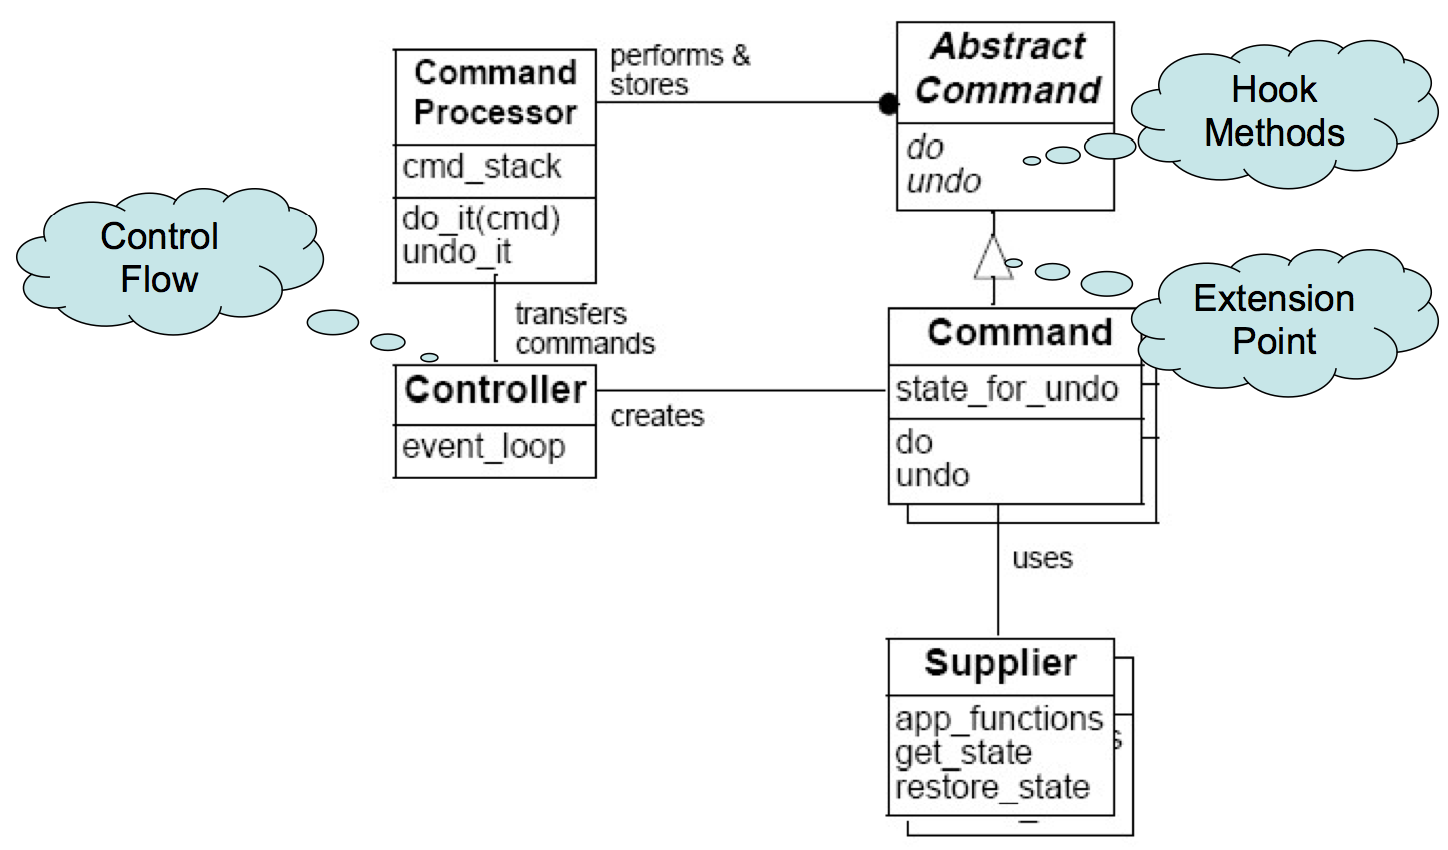
\includegraphics[width=0.9\textwidth]{content/frameworks/commandprocessormicroframework.png}
		\caption{Command Processor als Microframework}
	\end{figure}
\end{itemize}